\section{A classification-based approach}
\subsection{Board detection}
\todo{TODO: corner point detection}
\subsection{Occupancy classification}
Empirical experiments showed that performing piece classification directly after detecting the four corner points with no intermediate step yields a large number of false positives, i.e. empty squares being classified as containing a chess piece.
\begin{figure}
    \centering
    \begin{subfigure}[b]{0.65\textwidth}
        \centering
        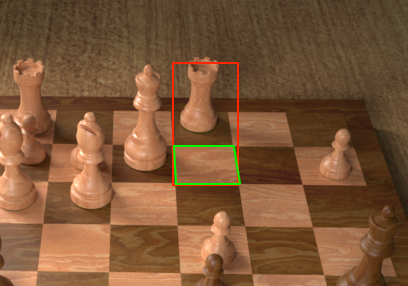
\includegraphics[width=\textwidth]{3828_annotated}
        \caption{region from the original image with marked square}
        \label{fig:occupancy_classification_fp_original}
    \end{subfigure}
    \hfill
    \begin{subfigure}[b]{0.3\textwidth}
        \centering
        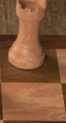
\includegraphics[width=.7\textwidth]{3828_cut}
        \caption{cropped sample}
        \label{fig:occupancy_classification_fp_cropped}
    \end{subfigure}
    \caption[An example illustraing why an immediate piece classification approach is inclined to reporting false positives.]{An example illustraing why an immediate piece classification approach is inclined to reporting false positives. Consider the square marked in green in the original image \subref{fig:occupancy_classification_fp_original}. The bounding box for piece classification (marked in red) must be quite tall because the square might contain a tall piece such as a queen or king (the box must be at least as tall as the the queen in the adjacent square on the left). The resulting sample, depicted in \subref{fig:occupancy_classification_fp_cropped}, contains almost the entire rook of the square behind. Thus, a piece classifier might classify this square as containing a rook instead of being empty.}
    \label{fig:occupancy_classification_fp}
\end{figure}
One common scenario where the trained classifier failed is illustrated in \cref{fig:occupancy_classification_fp}.
Notice that squares further away from the camera must be cropped with increasingly taller bounding boxes.
If a particular square is empty but its bounding box includes the piece from the adjacent square as in \cref{fig:occupancy_classification_fp_cropped}, the trained classifier was inclined to report a false positive.

To solve this problem, a binary classifier is trained on cropped squares to decide whether they are empty or not.
Before cutting out the squares from the original image, the input image is warped to a two-dimensional overhead view by means of a projective transformation.
This ensures that all squares are of equal size and that the corners form right angles (which is not the case in the original image due to perspective distortion).
To this end, we compute the \emph{homography matrix} $\mH \in \R^{3 \times 3}$ \cite{szeliski2011} mapping any point
$\vp$
from the original image to
the corresponding point
$\vp'$
in the warped image.
To simplify notation, we shall consider 2D homogenous coordinate vectors, i.e. three-component vectors with the last component being $1$, so the vector
$\begin{bmatrix}
    x & y & 1
\end{bmatrix}^\top$
would represent the point $(x,y)$ in the Cartesian coordinate system.
Using this notation, $\mH$ maps $\vp$ to $\vp'$ using the relation
\begin{equation}
    \label{eq:homography_matrix_relation}
    \mH
    \vp
    = s \vp'
\end{equation}
up to a scalar scale factor $s$.

Let the $4 \times 3$ matrix $\mP$ contain the pixel coordinates of the four chessboard corners starting in the top left in clockwise order and $\mP'$ be a matrix of the same size containing the corner coordinates of a square with side length $l$ pixels given by
\begin{equation*}
    \mP' = \begin{bmatrix}
        0 & l & l & 0 \\
        0 & 0 & l & l \\
        1 & 1 & 1 & 1
    \end{bmatrix}.
\end{equation*}
Notice that $\mP'$ describes a square whose top left corner is at the origin, and the coordinates are given in the same order as in $\mP$.
Since the homography matrix should map points from the original image to the output image, we obtain from \cref{eq:homography_matrix_relation} the relation 
\begin{equation}
    \label{eq:homography_matrix_relation_corners}
    \mH \mP = \mP' (\mI_4 \vs)
\end{equation}
where the vector $\vs \in \R^4$ represents the scale factor for each point.
\Cref{eq:homography_matrix_relation_corners} describes an overdetermined set of linear equations, so it is likely that there is no exact solution for $\mH$. 
However, we approximate $\mH$ by finding the solution with the least squared error.
Finally, we can use $\mH$ to apply the projective transformation to the original image such as depicted in \cref{fig:occupancy_classification_samples_original}, obtaining the warped image in \cref{fig:occupancy_classification_samples_warped}.
\begin{figure}
    \centering
    \begin{subfigure}[b]{0.47\textwidth}
        \centering
        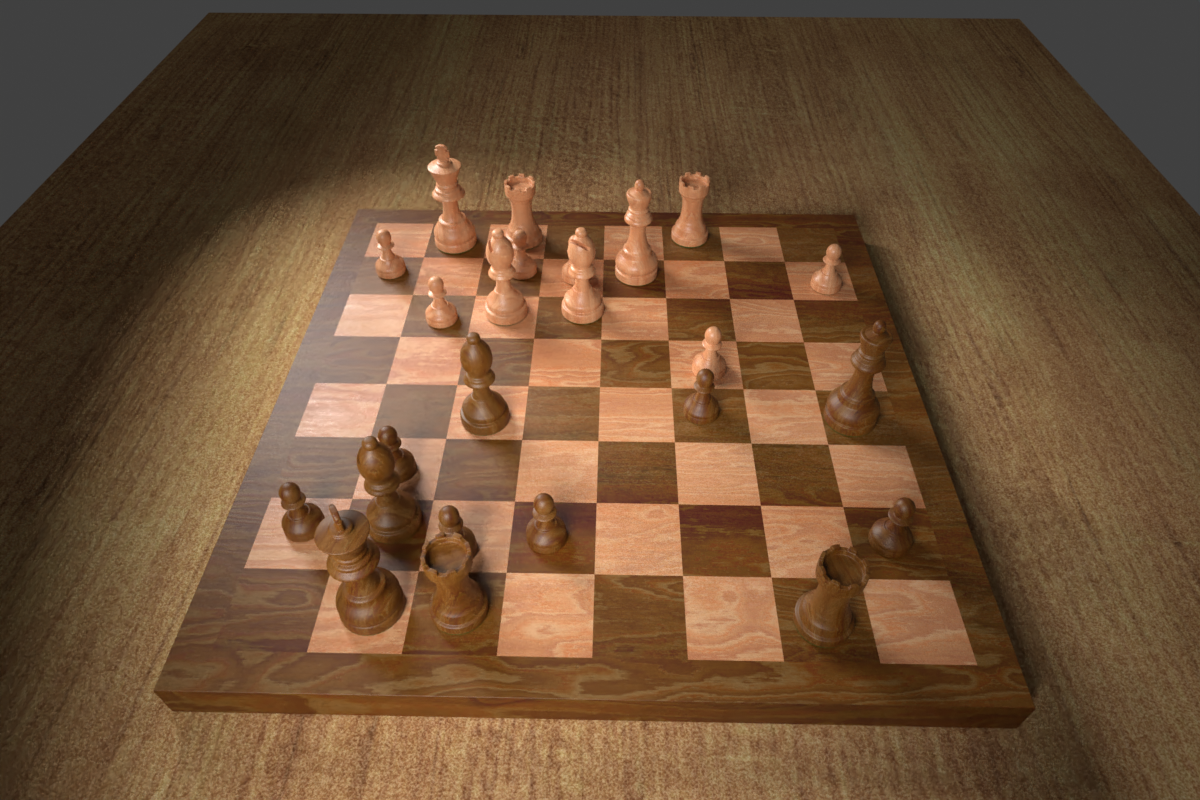
\includegraphics[width=\textwidth]{3828}
        \caption{original}
        \label{fig:occupancy_classification_samples_original}
    \end{subfigure}
    \hfill
    \begin{subfigure}[b]{0.47\textwidth}
        \centering
        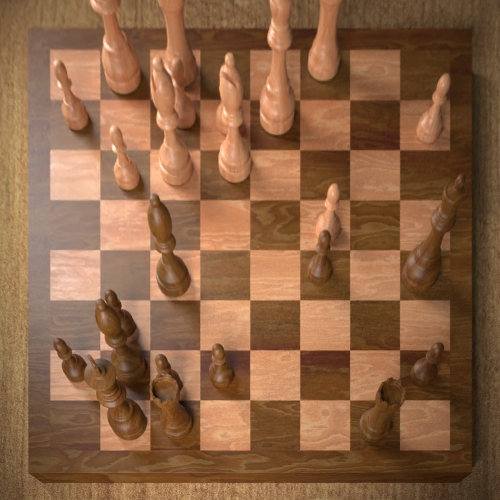
\includegraphics[width=\textwidth]{3828_unwarped}
        \caption{warped}
        \label{fig:occupancy_classification_samples_warped}
    \end{subfigure}
    
    \bigskip
    \begin{subfigure}[b]{0.47\textwidth}
        \centering
        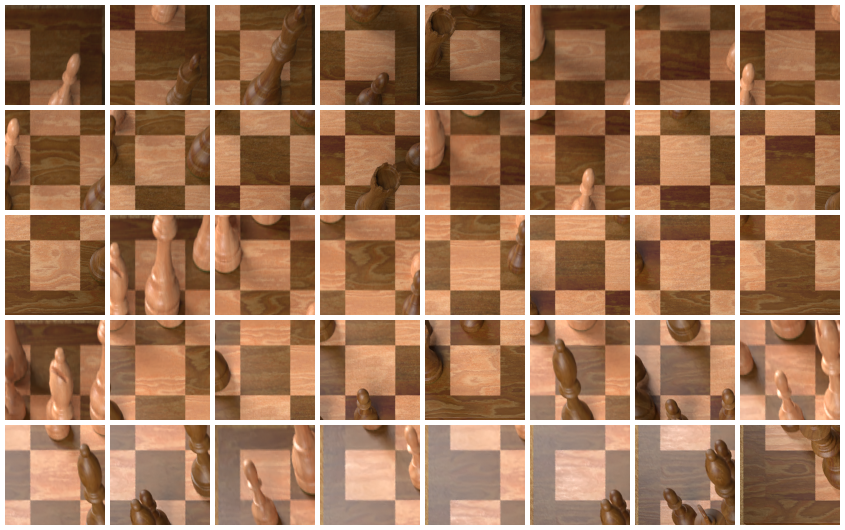
\includegraphics[width=\textwidth]{3828_empty}
        \caption{all 32 empty samples}
        \label{fig:occupancy_classification_samples_empty}
    \end{subfigure}
    \hfill
    \begin{subfigure}[b]{0.47\textwidth}
        \centering
        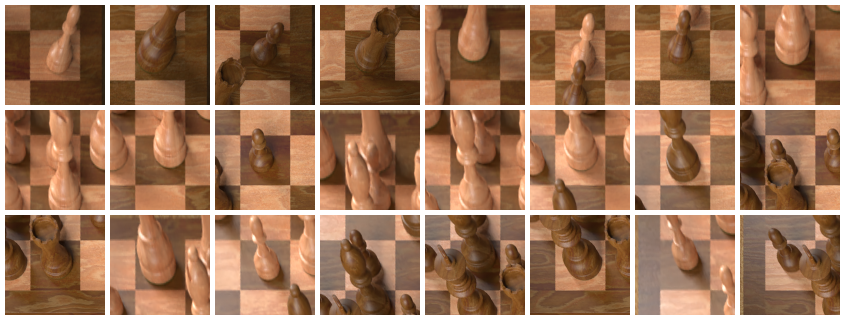
\includegraphics[width=\textwidth]{3828_occupied}
        \caption{all 24 occupied samples}
        \label{fig:occupancy_classification_samples_occupied}
    \end{subfigure}
    \caption[The process of obtaining samples for occupancy classification from a chessboard image.]{The process of obtaining samples for occupancy classification from a chessboard image. First, the original image \subref{fig:occupancy_classification_samples_original} is warped to a two-dimensional overhead view, \subref{fig:occupancy_classification_samples_warped}. Then, all squares are cropped (with a 50\% increase in width and height to include contextual information). Finally, the cropped squares are annoted using the \gls{fen} groundtruth as either empty \subref{fig:occupancy_classification_samples_empty} or occupied \subref{fig:occupancy_classification_samples_occupied}.}
    \label{fig:occupancy_classification_samples}
\end{figure}

Cropping the squares from the warped image is trivial because the squares are of equal size.
In training the occupancy classifiers, it is conjectured that it would be useful to include contextual information with each square; therefore, the squares are not cropped tightly around their boundaries but instead with a 50\% increase in length on all four sides, as shown in \cref{fig:occupancy_classification_samples_empty,fig:occupancy_classification_samples_occupied}.
This might aid the classifier's decision in difficult situations where a chess piece from another square reaches into the cropped one due to the camera perspective.

\subsubsection{\Glspl{cnn}}
Six \gls{cnn} architectures are devised for the occupancy classification task, of which two accept $100\times 100$ pixel input images and the remaining four require the images to be of size $50\times 50$ pixels.
They differ in the number of convolution layers, pooling layers, and fully connected layers.
When referring to these models, we will use a 4-tuple consisting of the input side length and the three aforementioned criteria.
\Cref{fig:occupancy_convnet} depicts the architecture of the \gls{cnn} $(100, 3, 3, 3)$ model which achieves the greatest validation accuracy of these six models.
\begin{figure}
    \centering
    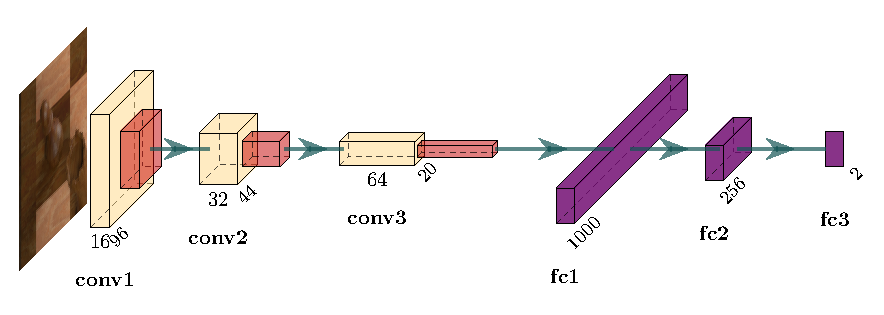
\includegraphics[width=\textwidth]{occupancy_convnet}
    \caption[Architecture of the CNN $(100,3,3,3)$ network for occupancy classification.]{
        Architecture of the \gls{cnn} $(100,3,3,3)$ network for occupancy classification.
        The input is a three-channel \gls{rgb} image with $100\times 100$ pixels.
        There are three convolutional layers (yellow) with a kernal size of $5 \times 5$ and stride $1$, meaning that each convolutional layer reduces the width and height by $4$.
        The first convolutional layer has 16 filters, and with each layer, the number of channels is doubled, as is common practice in \glspl{cnn} \cite{simonyan2015}.
        Each convolutional layer uses the \gls{relu} activation function and is followed by a max pooling layer with a $2\times 2$ kernel that is moved with a stride of $2$ such that the width and height are halved.
        Finally, the output of the last pooling layer is reshaped to a 640,000-dimensional vector that passes through two fully connected \gls{relu}-activated layers before reaching the final fully connected layer with softmax activation.
    }
    \label{fig:occupancy_convnet}
\end{figure}
The final fully connected layer in each model contains two output units that represent the two classes (occupied and empty).
The models are trained using the cross-entropy loss function on the outputs.
Training proceeds using the popular \emph{Adam} optimizer \cite{kingma2017} with a learning rate of $0.001$ for three whole passes over the training set using a batch size of 128.
After every 100 steps, the model's loss and accuracy is computed over the entire validation set, the results of which are reported in \cref{fig:occupancy_cnn_loss_accuracy}.
\begin{figure}
    \makebox[\textwidth][c]{
        \begin{subfigure}{.45\textwidth}
            \begin{tikzpicture}
                \begin{axis}[
                    no markers,
                    xlabel={step},
                    ylabel={cross-entropy loss},
                    title={Loss},
                    scale only axis,
                    width=.9\textwidth,
                    legend style={at={(0.98,0.98)},anchor=north east}
                ]
                    \addplot table [x=Step, y=Value, col sep=comma] {data/run-occupancy_classifier_CNN100_3Conv_3Pool_3FC_train-tag-Loss.csv};
                    \addplot table [x=Step, y=Value, col sep=comma] {data/run-occupancy_classifier_CNN100_3Conv_3Pool_3FC_val-tag-Loss.csv};
                    \legend{training,validation}
                \end{axis}
            \end{tikzpicture}
        \end{subfigure}
        \hfill
        \begin{subfigure}{.45\textwidth}
            \begin{tikzpicture}
                \begin{axis}[
                    no markers,
                    xlabel={step},
                    ylabel={accuracy},
                    title={Accuracy},
                    scale only axis,
                    width=.9\textwidth,
                    ylabel near ticks,
                    yticklabel pos=right,
                    legend style={at={(0.98,0.02)},anchor=south east}
                ]
                    \addplot table [x=Step, y=Value, col sep=comma] {data/run-occupancy_classifier_CNN100_3Conv_3Pool_3FC_train-tag-Accuracy.csv};
                    \addplot table [x=Step, y=Value, col sep=comma] {data/run-occupancy_classifier_CNN100_3Conv_3Pool_3FC_val-tag-Accuracy.csv};
                    \legend{training,validation}
                \end{axis}
            \end{tikzpicture}
        \end{subfigure}
    }
    \caption[Loss and accuracy during training on both the training and validation sets for the CNN $(100,3,3,3)$ model.]{Loss and accuracy during training on both the training and validation sets for the \gls{cnn} $(100,3,3,3)$ model. The best validation accuracy is 99.71\%.}
    \label{fig:occupancy_cnn_loss_accuracy}
\end{figure}
The model converges smoothly to a very low loss value, achieving a training accuracy of 99.70\% and validation accuracy of 99.71\%.
Due to the fact that the difference between training and validation accuracy is very small (in fact, the validation accuracy even happens to be slightly above the training accuracy), we conclude that the model does not overfit the training set.

\subsubsection{Transfer learning on deeper models}
\todo{todo: explain how this was done and explain tradeoff (significantly more parameters in model)}

Each model is trained separately on the dataset of squares that are cropped to include contextual information (by increasing the bounding box by 50\% in each direction), and the same samples except that the squares are cropped tightly.
In each case, the model trained on the samples that contained contexual information outperfomed its counterpart trained on tightly cropped samples, confirming the hypothesis that the information around the square itself is useful.


\begin{table}
    \centering
    \makebox[\textwidth][c]{
        \pgfplotstabletypeset[
            col sep=tab,
            columns={context,model,parameters,val_accuracy,val_precision/occupied,val_recall/occupied,val_misclassified,train_accuracy},
            every head row/.style={%
                before row=\toprule,
                after row=\midrule%
            },
            every last row/.style={
                after row=\bottomrule
            },
            columns/model/.style={
                string type
            },
            columns/context/.style={
                string type,
                column name={}
            },
            columns/val_accuracy/.style={
                dec sep align,
                postproc cell content/.append code={
                    \ifnum1=\pgfplotstablepartno
                        \pgfkeysalso{@cell content/.add={}{\%}}%
                    \fi
                },
                fixed,
                fixed zerofill,
                column name={accuracy}
            },
            columns/train_accuracy/.style={
                dec sep align,
                postproc cell content/.append code={
                    \ifnum1=\pgfplotstablepartno
                        \pgfkeysalso{@cell content/.add={}{\%}}%
                    \fi
                },
                fixed,
                fixed zerofill,
                column name={\makecell{training \\ accuracy}}
            },
            columns/val_precision/occupied/.style={
                dec sep align,
                precision=3,
                fixed,
                fixed zerofill,
                column name={precision}
            },
            columns/val_recall/occupied/.style={
                dec sep align,
                precision=3,
                fixed,
                fixed zerofill,
                column name={recall}
            },
            columns/val_misclassified/.style={
                column name={\makecell{errors}}
            },
        ]{data/occupancy_classifier.dat}
    }
    \caption[Performance of all occupancy classification models on the validation set.]{
        Performance of all occupancy classification models on the validation set.
        For the \gls{cnn} models, the 4-tuple denotes the length of the square input size in pixels, the number of convolution layers, the number of pooling layers, and the number of fully connected layers.
        The check mark in the left column indicates whether the input samples contained contextual information (cropped to include part of the adjacent squares).
        In the penultimate column, the total number of misclassifications in the validation set are reported (the validation set consists of 9,346 samples).
        The training accuracy is given in the rightmost column for comparison.
        Notice that there is no significant difference between the validation and training accuracies, indicating that none of the models suffer from overfitting.
    }
\end{table}

\begin{figure}
    \makebox[\textwidth][c]{
        \begin{subfigure}{.45\textwidth}
            \begin{tikzpicture}
                \begin{axis}[
                    no markers,
                    xlabel={step},
                    ylabel={cross-entropy loss},
                    title={Loss},
                    scale only axis,
                    width=.9\textwidth,
                    legend style={at={(0.98,0.98)},anchor=north east}
                ]
                    \addplot table [x=Step, y=Value, col sep=comma] {data/run-occupancy_classifier_ResNet_train-tag-Loss.csv};
                    \addplot table [x=Step, y=Value, col sep=comma] {data/run-occupancy_classifier_ResNet_val-tag-Loss.csv};
                    \legend{training,validation}
                \end{axis}
            \end{tikzpicture}
        \end{subfigure}
        \hfill
        \begin{subfigure}{.45\textwidth}
            \begin{tikzpicture}
                \begin{axis}[
                    no markers,
                    xlabel={step},
                    ylabel={accuracy},
                    title={Accuracy},
                    scale only axis,
                    width=.9\textwidth,
                    ylabel near ticks,
                    yticklabel pos=right,
                    legend style={at={(0.98,0.02)},anchor=south east}
                ]
                    \addplot table [x=Step, y=Value, col sep=comma] {data/run-occupancy_classifier_ResNet_train-tag-Accuracy.csv};
                    \addplot table [x=Step, y=Value, col sep=comma] {data/run-occupancy_classifier_ResNet_val-tag-Accuracy.csv};
                    \legend{training,validation}
                \end{axis}
            \end{tikzpicture}
        \end{subfigure}
    }
    \caption[Loss and accuracy during training on both the training and validation sets for the ResNet model.]{Loss and accuracy during training on both the training and validation sets for the ResNet model. The best validation accuracy is 99.96\%.}
    \label{fig:occupancy_resnet_loss_accuracy}
\end{figure}

\begin{figure}
    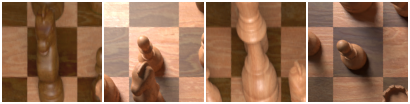
\includegraphics[width=\textwidth]{ResNet_val_mistakes.png}
    \caption[The four samples that the ResNet model misclassified in the validation set.]{The four samples that the ResNet model misclassified in the validation set. The left sample depicts an empty square, and the three other samples are of occupied squares.}
    \label{fig:occupancy_resnet_mistakes}
\end{figure}

\subsection{Piece classification}